% this TeX file provides an awesome example of how TeX will make super 
% awesome tables, at the cost of your of what happens when you try to make a
% table that is very complicated.
% Originally turned in for Dr. Nico's Security Class
\documentclass[11pt]{article}


\usepackage[a4paper,margin=2cm]{geometry}
\usepackage{graphicx}
\usepackage{float}

\usepackage{amsmath}

\usepackage[makeroom]{cancel} %for crossing out terms in equations

\usepackage{todonotes}




% Use wide margins, but not quite so wide as fullpage.sty
%\marginparwidth 0.2in 
%\oddsidemargin 0.25in 
%\evensidemargin 0.25in 
%\marginparsep 0.25in
%\topmargin 0.25in 
%\textwidth 6in \textheight 8 in
% That's about enough definitions

\usepackage{listings}
\usepackage{url}
\usepackage{todonotes}
\begin{document}
% this is an alternate method of creating a title
%\hfill\vbox{\hbox{Gius, Mark}
%       \hbox{Cpe 456, Section 01}  
%       \hbox{Lab 1}    
%       \hbox{\today}}\par
%
%\bigskip
%\centerline{\Large\bf Lab 1: Security Audit}\par
%\bigskip
\author{
Rhys Agombar \\ 
Thiago Bell Felix de Oliveira
}
\title{Computer Vision - Sheet 1}
\maketitle

\section*{Question 3}
\noindent
\begin{figure}[H]
 
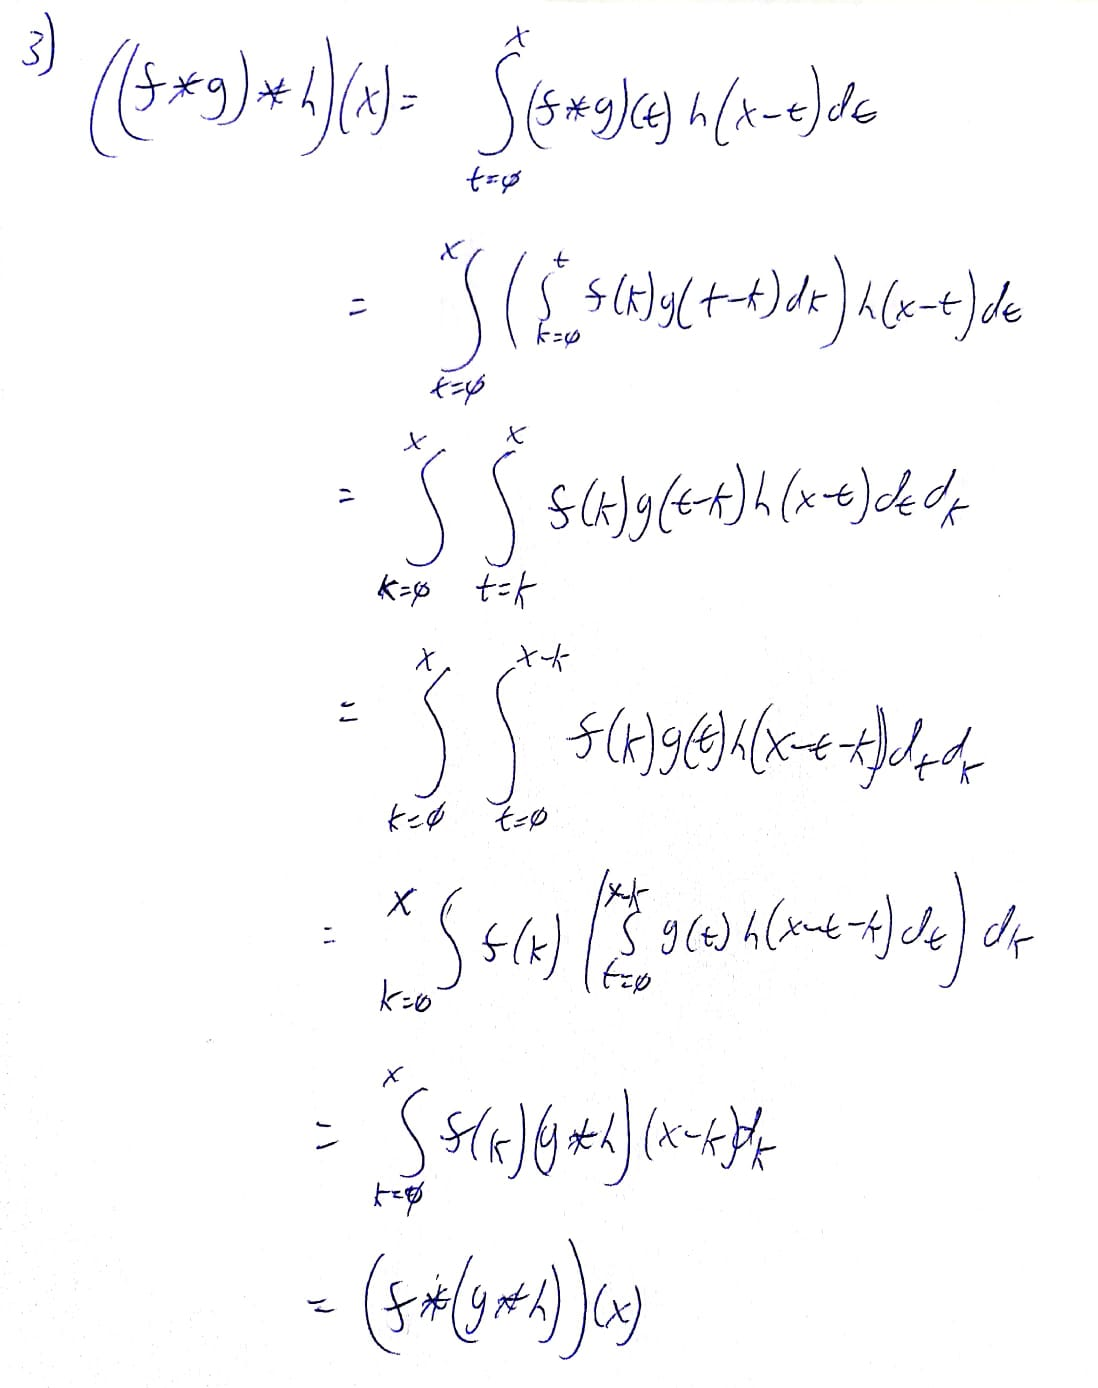
\includegraphics[width=0.8\linewidth]{q3img}

\end{figure}

\section*{Question 6}
\noindent
The Fourier Transform of a gaussian is another gaussian:
\begin{equation}
 FT(G(x,\sigma) = \frac{\sqrt{2\pi}}{\sigma} G(w, \sigma^{-1})
\end{equation}

A convoltion in the space domain is a multiplication is the frequency one:

\begin{equation}
G(x,\sigma)*G(x,\sigma) =  \left( \frac{\sqrt{2\pi}}{\sigma} G(w, \sigma^{-1}) \right)  ^2
\end{equation}

Therefore, two convolutions with the standard deviation $\sigma$ is equivalent to a convolution of standard deviation $\sigma'$:

\begin{equation}
 \frac{\cancel{2\pi}}{\cancel{\sigma^2}} \left( \frac{1}{\cancel{2\pi\sigma^{-2}}} e^{\frac{-x^2}{\sigma^{-2}}}  \right) =  \frac{\sqrt{2\pi}}{\sigma'} G(w, {\sigma'}^{-1})
\end{equation}

\begin{equation}
 e^{\frac{-x^2}{\sigma^{-2}}} = \frac{\cancel{\sqrt{2\pi}}}{\cancel{\sigma'}} \frac{1}{\cancel{\sqrt{2\pi}}\cancel{{\sigma'}^{-1}}} e^{\frac{-x^2}{2({\sigma'}^{-1})^2}}
\end{equation}

\begin{equation}
 e^{\frac{-x^2}{\sigma^{-2}}} = e^{\frac{-x^2}{2 (   {{\sigma'}^{-1}  })^2     }}
\end{equation}

\begin{equation}
 \sigma^{-2} = 2 ({\sigma'}^{-1})^2
\end{equation}

\begin{equation}
 \sigma^{-1} = \sqrt{2} {\sigma'}^{-1}
\end{equation}

\begin{equation}
 \sigma\sqrt{2} = \sigma'
\end{equation}

So, applying two convolutions with std. dev of $\sigma$ is the same as applying once with $\sigma\sqrt{2}$

\end{document}
